\documentclass[11pt]{scrartcl}
\usepackage[sexy]{evan}
\usepackage[a4paper, portrait, margin=0.75in]{geometry}
\usepackage{pxfonts}
\usepackage{anyfontsize}
\renewcommand*{\sfdefault}{cmss}
\usepackage{cases}
\usepackage{multirow}

\definecolor{ChadDarkBlue}{rgb}{.1,0,.2}  
\definecolor{ChadBlue}{rgb}{.1,.1,.5}  
\definecolor{ChadRoyal}{rgb}{.2,.2,.8}  
%\definecolor{ChadGreen}{rgb}{0,.35,.1}
%\definecolor{ChadGreen}{rgb}{0,.5,.25}  % Too bright
%\definecolor{ChadGreen}{rgb}{0,.4,.2}    % Still too bright
\definecolor{ChadGreen}{rgb}{0.5, 0, 0.2}    % Dark Green
%\definecolor{ChadRed}{rgb}{.8,.1,.2}    % Too bright
\definecolor{ChadRed}{rgb}{.5,0,.5}  % purple
\title{Young Modulus \& Error Analysis}

\begin{document}
\begin{titlepage}
    \begin{center}
        \sffamily

        \vspace*{1cm}
        
        \huge
        \color{darkgray}{\textbf{PH1102: Experiment I}}

        \vspace{0.5cm}

        \Huge
        {\color{ChadBlue}{\textbf{Retrieving Young Modulus \& \\
        A Glimpse on Error Analysis}}}
            
        \vspace{0.5cm}
        \LARGE
        \color{darkgray}{\normalfont{Laboratory Report}}
            
        \vspace{1.5cm}
            
        {\color{ChadGreen}{\textbf{Abhisruta Maity, 21MS006 \plusemail{am21ms006@iiserkol.ac.in}}}}
            
        \vfill

        
\includegraphics[scale=0.08]{IISER-K_Logo.png}
            
        \vspace{0.8cm}
            
        \color{ChadBlue}{\Large
        {\normalfont{Department of Physical Sciences\\
        \emph{Indian Institute of Science Education and Research, Kolkata}\\
        India\\
        \today}}}
            
    \end{center}
\end{titlepage}

\section{Introduction}
\fontsize{12}{18}\selectfont
Analogous to the density of a substance, the \emph{Young's modulus} of a solid object determines the quantitative measure of its strength, elasticity, and some other intrinsic materialistic properties. By this experiment, done in PH1102, we try to deduce the young modulus of a solid metal bar by the \emph{flexure method}. Though its `behind-the-scene' formula is quite tricky and intimidating, it is very convenient for practical purposes. Also, to understand experimental accuracy, we have done a brief error analysis playing with the given dataset and a little bit of statistical computation.

\section{Aim of the Experiment}
To determine Young's modulus of a metal bar by the flexure method.

\section{Principle and Working Formula}
A metal bar is kept horizontal with two knife-edge support at the two ends. When different suitable weights are fixed at the middle point of the bar, it gets depressing (Fig. \ref{fig:bar1}). The amount of depression \(d\) is related to Young's modulus \(Y\) of the bar material. By experimentally measuring length, breadth, and thickness of the bar and depression \(d\) for different weights \(W\), Young's modulus \(Y\) can be determined.

\begin{figure}[h]
    \centering
    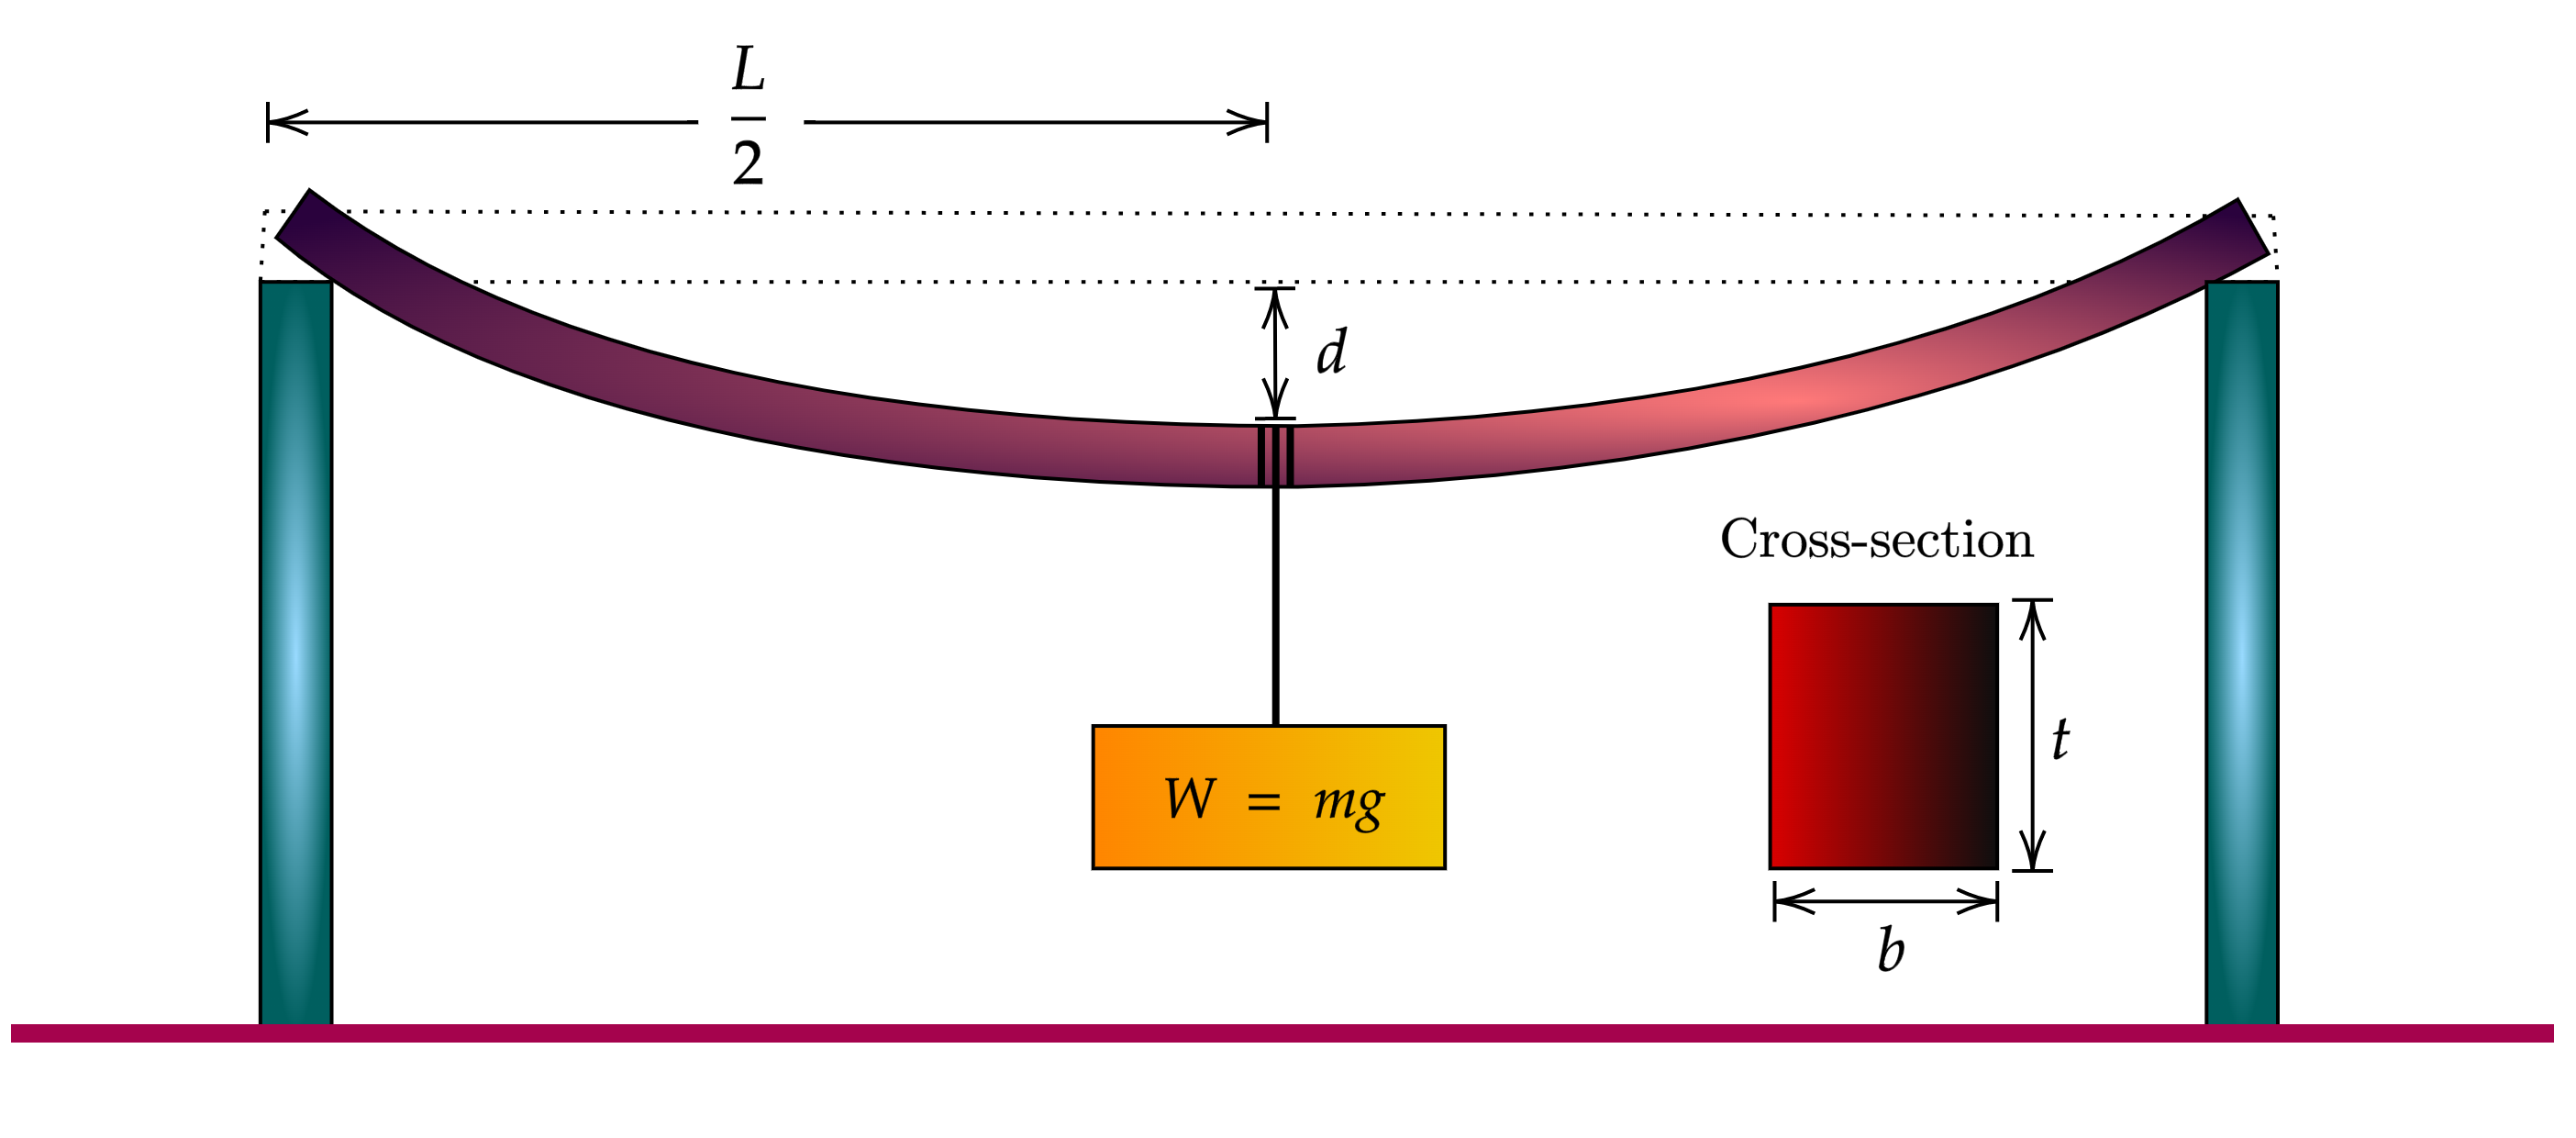
\includegraphics[scale=0.15]{diagram-20220212 (1).png}
    \caption{The experimental set-up and the cross-section of the bar}
    \label{fig:bar1}
\end{figure}

The bar in Fig. 1 can be regarded as two cantilevers, each of length \(\frac{L}{2}\),
fixed at the center (where weight is hanged) and loaded by \(\frac{W}{2}\) at the
two knife-edges. Each cantilever undergoes depression \(d\) given by 
\begin{equation}
    d = \frac{WL^3}{4Ybt^3} = \frac{mgL^3}{4Ybt^3} \implies Y = \frac{mgL^3}{4bdt^3}
\end{equation}
Actually, it is difficult to know the absolute value of depression, because, even without any additional weight, the bar will be
depressed slightly due to its own weight. So, one measures relative depression as a function of added weights and plots a graph:
\(d\) vs. \(m\), which is a straight line with a slope
\[s = \frac{gL^3}{4Ybt^3}\]
From the slope \(s\) of the \(d\) vs. \(m\) graph one can calculate Young's
modulus as
\begin{equation}
    \boxed{Y = \frac{gL^3}{4sbt^3}}
    \label{eqn:main}
\end{equation}

\section{Procedure}
\begin{enumerate}
    \item Measure the breadth \(b\) of the bar using a Vernier caliper and tabulate the data.
    \item Measure the thickness \(t\) of the bar using a screw gauge and tabulate the data.
    \item Measure the length \(L\) of bar between two knife-edges i.e. separation between two knife-edges (Fig. \ref{fig:bar1}) using a meter scale and tabulate the data.
    \item Mark the point on the bar exactly at the center of the two knife-edges. Put the hanger of the weights exactly at that point. The hanger has pointer on top.
    \item Focus the travelling microscope such that the pointer is clearly seen in it. Position the travelling microscope such that the pointer is touching the horizontal cross wire. Note down the reading of the vertical scale of the travelling microscope.
    \item Add one weight block on the hanger. Mass of all the weight blocks should be already written on them. If it is missing, weigh the block and write it down. The bar will depress and the pointer will move in the microscope field of view. Adjust microscope vertical position to align the pointer back to the horizontal cross wire. Note the reading of the vertical scale of the travelling microscope. 
    \item Similarly, note microscope reading for addition of 4-5 more weight blocks one after another.
    \item Then start reducing the weight one by one and each time adjust microscope to align the pointer at the horizontal cross wire and take microscope reading till the hanger is empty again. 
    \item Record data for steps 5-8 in a table. Calculate average depression \(d\) for a given amount of mass \(m\) on the hanger.
\end{enumerate}

\newpage

\section{Dataset Manipulation}
By proceeding along the methods above, we found: \(L = 86\) cm. And we are given: Least count of the screw gauge \(= 0.001\) cm and Vernier constant \(=0.002\) cm. Then we proceed to find \(b, t\) and \(d\).

\begin{table}[h]
    \def\arraystretch{1.25}
    \centering
    \caption{Determination of the breadth of the bar \(b\) using Vernier Caliper}

    \vspace{0.5em}

    \begin{tabular}{|c|c|c|c|c|c|}
    \hline
    Sl. No. &
      \begin{tabular}[c]{@{}c@{}}MSR\\ (cm)\end{tabular} &
      VSR &
      \begin{tabular}[c]{@{}c@{}}VC\\ (cm)\end{tabular} &
      \begin{tabular}[c]{@{}c@{}}Breadth \(b\)\\ {[}MSR + (VSR \(\times\) VC){]}\\ (cm)\end{tabular} &
      \begin{tabular}[c]{@{}c@{}}Average Breadth\\ (cm)\end{tabular} \\ \hline
    1 & 2.5 & 40 & 0.002 & 2.58  &      \\ \cline{1-5}
    2 & 2.5 & 16 & 0.002 & 2.532 & 2.55 \\ \cline{1-5}
    3 & 2.5 & 25 & 0.002 & 2.55  &      \\ \hline
    \end{tabular}
\end{table}

\vspace{0.5em}

\begin{table}[h]
    \def\arraystretch{1.25}
    \centering
    \caption{Determination of the thickness of the bar \(t\) using Screw Gauge}

    \vspace{0.5em}

    \begin{tabular}{|c|c|c|c|c|c|}
    \hline
    Sl. No. &
      \begin{tabular}[c]{@{}c@{}}LSR\\ (cm)\end{tabular} &
      CSR &
      \begin{tabular}[c]{@{}c@{}}LC\\ (cm)\end{tabular} &
      \begin{tabular}[c]{@{}c@{}}Thickness \(t\)\\ {[}LSR + (CSR \(\times\) LC){]}\\ (cm)\end{tabular} &
      \begin{tabular}[c]{@{}c@{}}Average Thickness\\ (cm)\end{tabular} \\ \hline
    1 & 4.5 & 41 & 0.001 & 4.91  &      \\ \cline{1-5}
    2 & 4.5 & 36 & 0.001 & 4.86  & 4.88 \\ \cline{1-5}
    3 & 4.5 & 38 & 0.001 & 4.88  &      \\ \hline
    \end{tabular}
\end{table}

\vspace{0.5em}

\begin{table}[h]
    \centering
    \def\arraystretch{1.25}
    \caption{Determination of Average Depression for Cumulative Loading and Unloading Mass}

    \vspace{0.5em}

    \begin{tabular}{|c|c|ccc|c|ccc|c|c|}
    \hline
    \multirow{2}{*}{\begin{tabular}[c]{@{}c@{}} Sl. \\ No. \\ (1 - 6) \end{tabular}} & \multirow{2}{*}{\begin{tabular}[c]{@{}c@{}}Mass on \\ hanger \\ \(m\) (g)\end{tabular}} & \multicolumn{3}{c|}{Loading} & \multirow{2}{*}{\begin{tabular}[c]{@{}c@{}} Dep. \\ \(d_1\) \\ (mm)\end{tabular}} & \multicolumn{3}{c|}{Unloading} & \multirow{2}{*}{\begin{tabular}[c]{@{}c@{}} Dep. \\ \(d_2\) \\ (mm)\end{tabular}} & \multirow{2}{*}{\begin{tabular}[c]{@{}c@{}}Average\\ Depression\\ \(\frac{d_1+d_2}{2}\) (mm)\end{tabular}} \\ \cline{3-5} \cline{7-9}
     &  & \multicolumn{1}{c|}{\begin{tabular}[c]{@{}c@{}}MSR\\ (mm)\end{tabular}} & \multicolumn{1}{c|}{VSR} & \begin{tabular}[c]{@{}c@{}}\(x_1\)\\ (mm)\end{tabular} &  & \multicolumn{1}{c|}{\begin{tabular}[c]{@{}c@{}}MSR\\ (mm)\end{tabular}} & \multicolumn{1}{c|}{VSR} & \begin{tabular}[c]{@{}c@{}}\(x_2\)\\ (mm)\end{tabular} &  &  \\ \hline
    1 & 0 & \multicolumn{1}{c|}{113} & \multicolumn{1}{c|}{20} & 113.20 & 0 & \multicolumn{1}{c|}{112.5} & \multicolumn{1}{c|}{40} & 112.90 & 0 & 0 \\ \hline
    2 & 426 & \multicolumn{1}{c|}{112} & \multicolumn{1}{c|}{33} & 112.33 & 0.9 & \multicolumn{1}{c|}{112} & \multicolumn{1}{c|}{5} & 112.05 & 0.9 & 0.9 \\ \hline
    3 & 908 & \multicolumn{1}{c|}{110.5} & \multicolumn{1}{c|}{25} & 110.75 & 2.5 & \multicolumn{1}{c|}{110.5} & \multicolumn{1}{c|}{15} & 112.65 & 2.3 & 2.4 \\ \hline
    4 & 1393 & \multicolumn{1}{c|}{109} & \multicolumn{1}{c|}{10} & 109.10 & 4.1 & \multicolumn{1}{c|}{109} & \multicolumn{1}{c|}{23} & 109.23 & 3.7 & 3.9 \\ \hline
    5 & 1883 & \multicolumn{1}{c|}{108} & \multicolumn{1}{c|}{5} & 108.05 & 5.2 & \multicolumn{1}{c|}{107.5} & \multicolumn{1}{c|}{30} & 107.80 & 5.1 & 5.1 \\ \hline
    6 & 2843 & \multicolumn{1}{c|}{105} & \multicolumn{1}{c|}{38} & 105.38 & 7.8 & \multicolumn{1}{c|}{105} & \multicolumn{1}{c|}{30} & 105.30 & 7.6 & 7.7 \\ \hline
    \end{tabular}
\end{table}
In the next section, we plot a graph of Depression \(d\) against mass on the hanger \(m\) and do some computation.

\newpage

\section{Computation: Linear Regression}
\begin{figure}[h]
    \centering
    \fbox{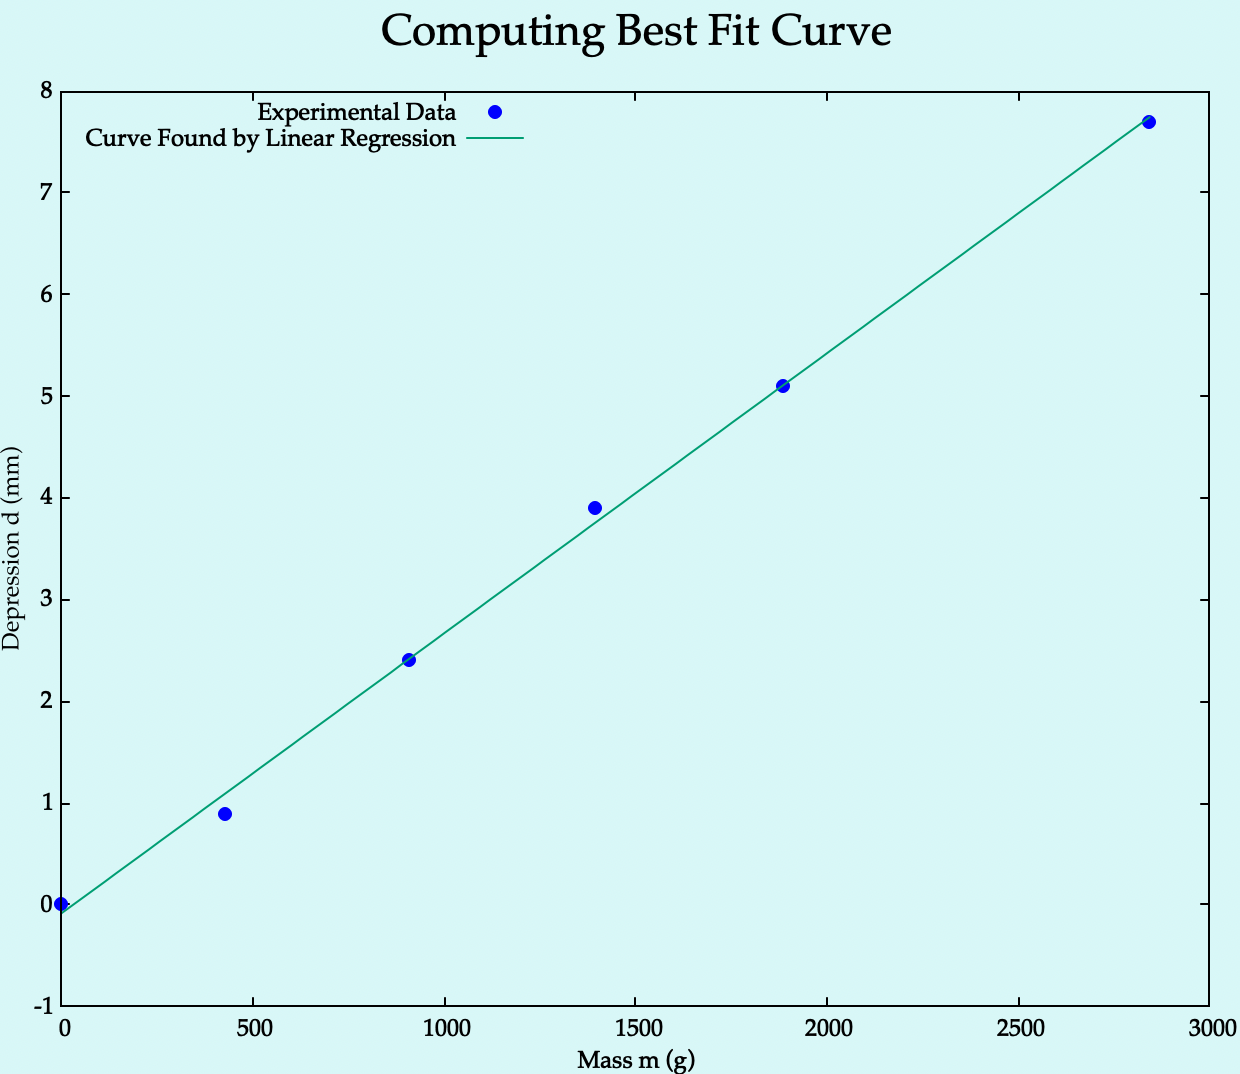
\includegraphics[scale=0.75]{Screenshot 2022-02-12 at 10.33.25 PM.png}}
    \caption{The graph of \(d\) vs. \(m\)}
\end{figure}

By exploring this computed graph, it really makes sense to have a quantity like Young's Modulus which is connected to the constant value of the slope.

This graph is plotted and the linear regression is computed using \texttt{gnuplot} in the terminal. After the computation, the terminal replied the following equation of the line 
\begin{equation}
    \boxed{y = 0.0027547x - 0.0884668}
\end{equation}
upto a `sufficient' number of significant figures.

Notice that, we have found the desired slope of the best fit line and that is \[s = 0.0027547 \text{ mm g}^{-1}\]

\begin{remark}
    Units are very impotant for any measure.
\end{remark}

\newpage

\section{Calculation of Young's Modulus}
From the above results, we summarise with standarizing their units: 
\begin{itemize}
    \item \(L = 86\) cm \(0.86\) m
    \item \(g = 9.8\) m s\(^{-2}\)
    \item \(b = 2.55\) cm \(= 0.255\) m
    \item \(t = 4.88\) mm \(= 0.00488\) m
    \item \(s = 0.0027547 \text{ mm g}^{-1} = 0.0027547 \text{ m kg}^{-1}\) 
\end{itemize}
Plugging these values to Equation \ref{eqn:main}, yields 
\begin{align}
    Y = \frac{9.8 \times 0.86^3}{4 \times 0.0027547 \times 0.0255 \times 0.00488^3} \text{ N m}^{-2} \approx \boxed{1.91 \times 10^{11} \text{ N m}^{-2}}
    \label{eqn:young}
\end{align}

\section{Error Analysis}
In this section, we talk about the statistical errors on doing linear regression and the experimental errors.
\subsection{Error in Regression}
After computing the best fit linear curve through \texttt{gnuplot}, the output went like this:
\begin{figure}[h]
    \centering
    \fbox{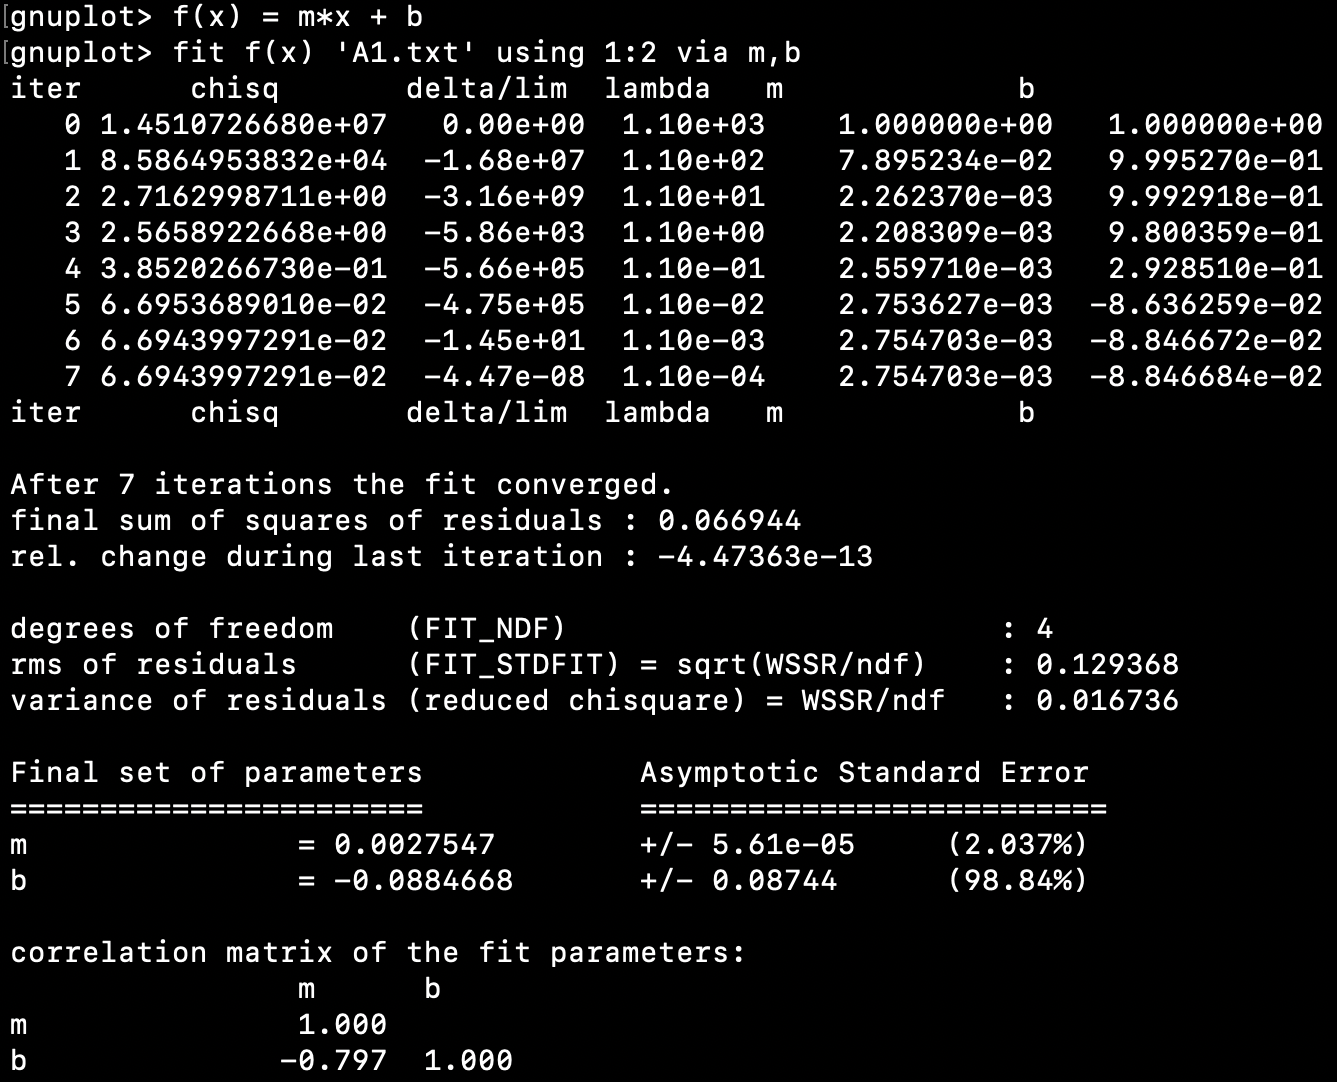
\includegraphics[scale=0.55]{Screenshot 2022-02-12 at 10.40.25 PM.png}}
    \caption{The output window of \texttt{gnuplot} after computation}
    \label{fig:gnuplot}
\end{figure}

\newpage

Fig. \ref{fig:gnuplot} contains some information about the errors in each data point \(y_i - y\) where the set \(\{(x_i, y_i) : i = 1, 2, \cdots 6\}\) represents all the points that we found from experimental dataset. These \(y_i - y\) are called \emph{residuals}. Computation yields their varience and standard deviation as \[\sigma^2 = 0.016736; \qquad \sigma = 0.129368\] Clearly, \(\sigma\) is quite low with respect to the \(y_i\)s. So the above linear regression is acceptable.

\subsection{Experimental Error}

The literature value of Young's Modulus (\(Y\)) of Steel\footnote{Source: \url{https://www.azom.com/article.aspx?ArticleID=6117}} \(= 2.00 \times 10^{11}\). Combining this with Equation \ref{eqn:young}, we calculate the error in \(Y\): \[\Delta Y = 2.00 \times 10^{11} - 1.91 \times 10^{11} \text{ N m}^{-2} = 0.09 \times 10^{11} \text{ N m}^{-2} \]
Then, percentage relative error in \(Y\): \[\% \frac{\Delta Y}{Y} = \frac{0.09 \times 10^{11} \text{ N m}^{-2}}{2.00 \times 10^{11} \text{ N m}^{-2}} \times 100 = 4.5\]
Observe that, \(4.5 \%\) of error is quite low for environments in general laboratories. This gives a hope to be more accurate next time we perform the experiment.

\section{Conclusion}
By this nice experiment, we quantitatively measured an intensive property of a material. We also got familiar with computation, curve fitting (i.e., regression), and some statistical entities. Error analysis is also important of any experiment, which we tried to briefly understand by this simple experiment in PH1102.

\section{Acknowledgements}
\textsc{Thanks} to the instructors of PH1102 for exposing us to IISER laboratories, handling experiments in this new era remotely and teaching how to perform computations in open-source \texttt{gnuplot} and Evan Chen, MIT for this beautiful \texttt{.sty} file for latexisation.
\end{document}